\begin{surferPage}[15 Keerpunten]{Een vijfdegraadsoppervlak met 15 keerpunten}
  Dit vijfdegraadsoppervlak heeft $15$ singulariteiten van het type $A_2$ (keerpunten genaamd); dit, en een aantal gerelateerde oppervlakken, werden beschreven in een artikel uit 2005 door Oliver Labs.
    Vijf van deze keerpunten zien er anders uit dan de overige tien.
    Die vijf zijn immers $A_2^{++}$-singulariteiten, de andere $A_2^{+-}$:

     \vspace*{-0.3em}
    \begin{center}
      \begin{tabular}{c@{\qquad}c}
        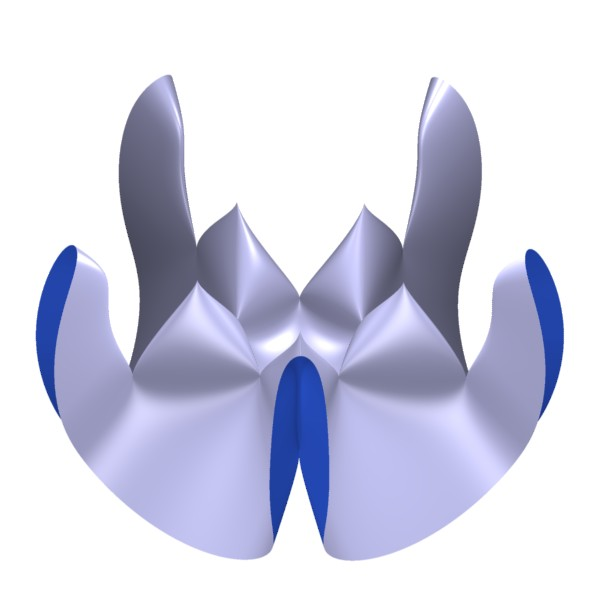
\includegraphics[height=1.2cm]{dessins_quint_15a2}
        &
        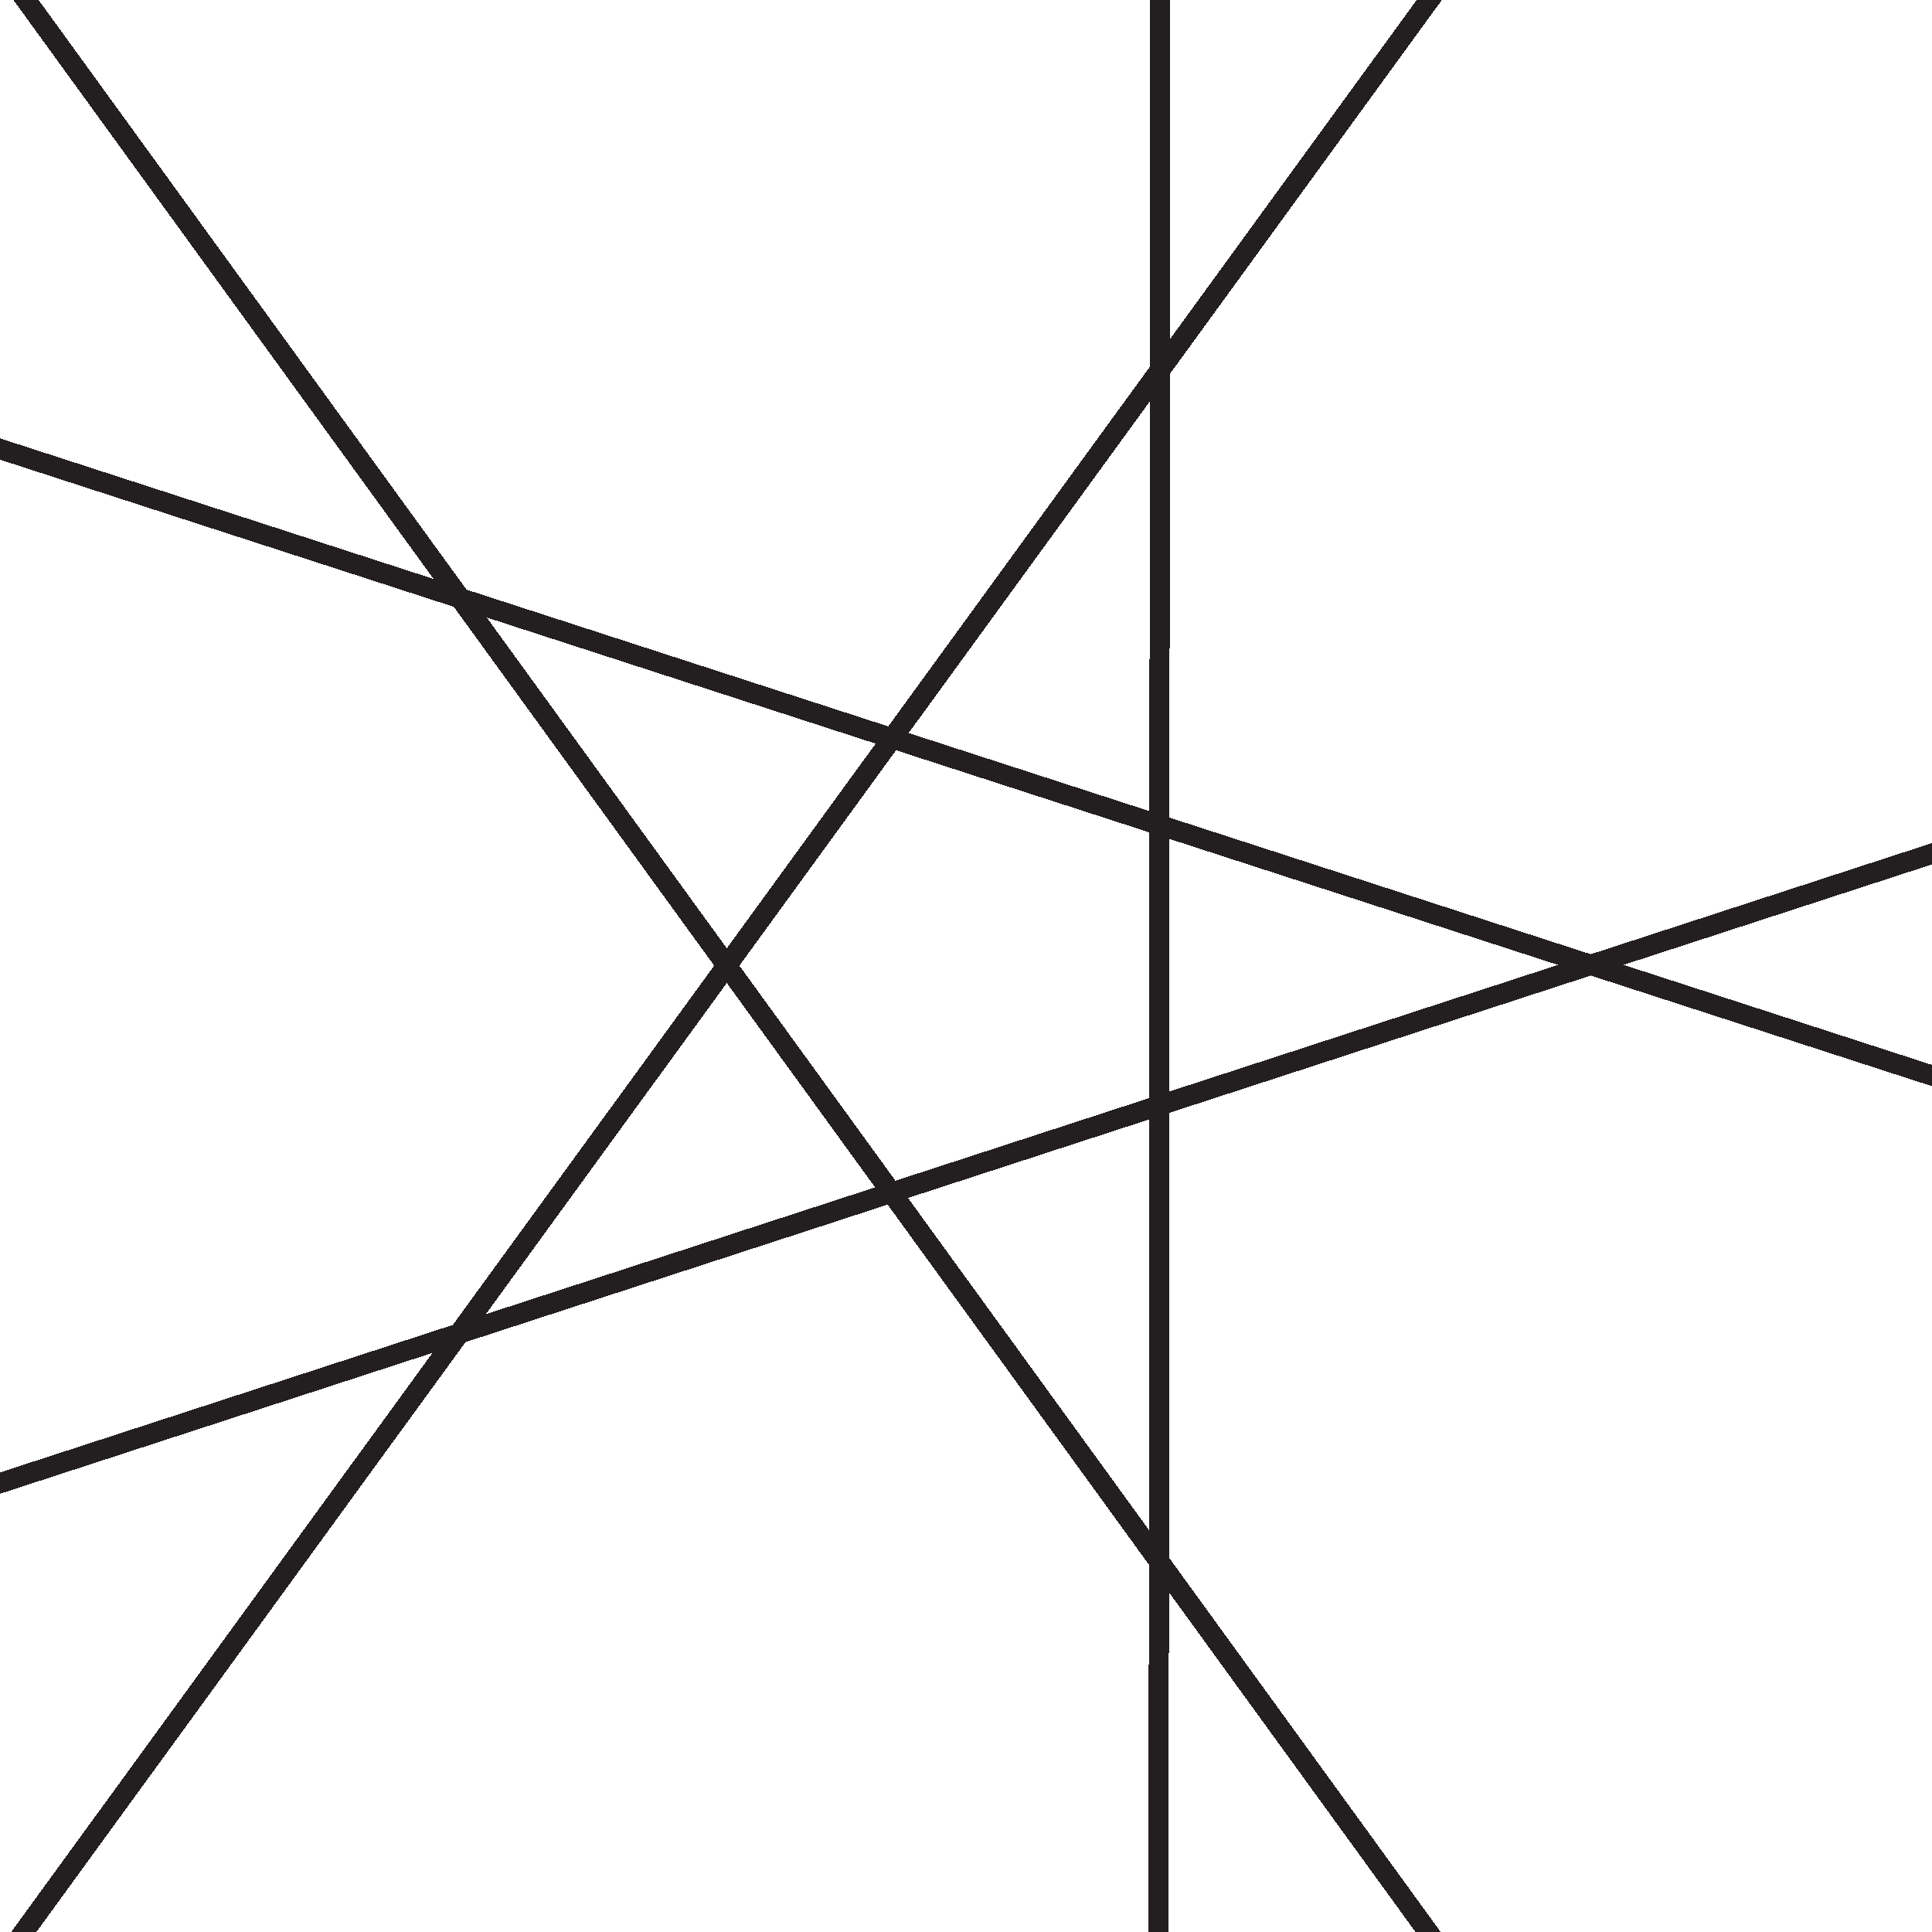
\includegraphics[height=1.2cm]{rp5.pdf}
      \end{tabular}
    \end{center}
    \vspace*{-0.3em}    
    
    Dit oppervlak heeft een vergelijking van de vorm
    $S_5(x,y) + t(z)=0,$
    waar $S_5(x,y)$ een regelmatige vijfhoek is (afbeelding rechts) en $t(z)$ een variant  is van de reeds vermelde Chebychev-veeltermen.

    Nog een vijfdegraadsoppervlak met $15$ keerpunten (links) werd geconstrueerd door Wolf Barth; ze is verwant met het derdegraadsoppvlak van Clebsch (rechts), zoals we op de middelste afbeelding kunnen zien:

    \vspace*{-0.3em}
    \begin{center}
      \begin{tabular}{c@{\quad}c@{\quad}c}
        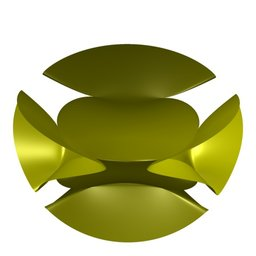
\includegraphics[height=1.2cm]{barthquintic_green}
        &
        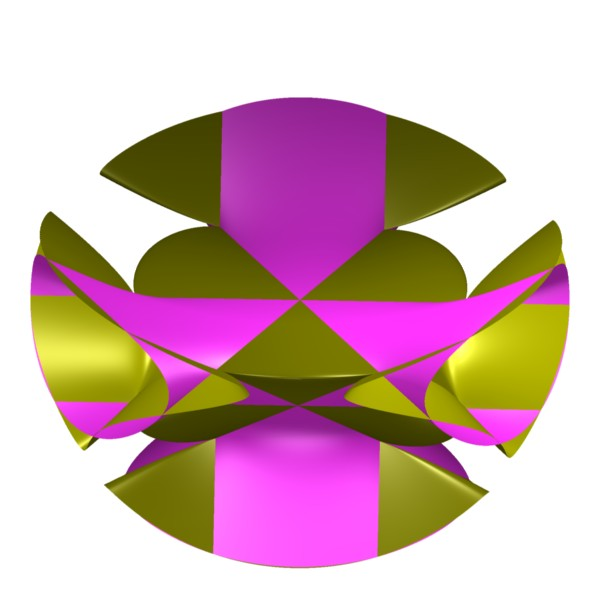
\includegraphics[height=1.2cm]{barthquintic_clebschcubic}
        &
        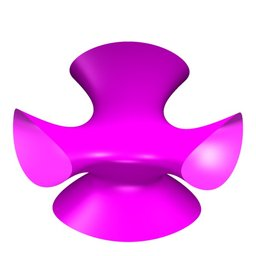
\includegraphics[height=1.2cm]{clebschcubic_pink}
      \end{tabular}
    \end{center}
    \vspace*{-0.3em}
\end{surferPage}
